\documentclass[1p]{elsarticle_modified}
%\bibliographystyle{elsarticle-num}

%\usepackage[colorlinks]{hyperref}
%\usepackage{abbrmath_seonhwa} %\Abb, \Ascr, \Acal ,\Abf, \Afrak
\usepackage{amsfonts}
\usepackage{amssymb}
\usepackage{amsmath}
\usepackage{amsthm}
\usepackage{scalefnt}
\usepackage{amsbsy}
\usepackage{kotex}
\usepackage{caption}
\usepackage{subfig}
\usepackage{color}
\usepackage{graphicx}
\usepackage{xcolor} %% white, black, red, green, blue, cyan, magenta, yellow
\usepackage{float}
\usepackage{setspace}
\usepackage{hyperref}

\usepackage{tikz}
\usetikzlibrary{arrows}

\usepackage{multirow}
\usepackage{array} % fixed length table
\usepackage{hhline}

%%%%%%%%%%%%%%%%%%%%%
\makeatletter
\renewcommand*\env@matrix[1][\arraystretch]{%
	\edef\arraystretch{#1}%
	\hskip -\arraycolsep
	\let\@ifnextchar\new@ifnextchar
	\array{*\c@MaxMatrixCols c}}
\makeatother %https://tex.stackexchange.com/questions/14071/how-can-i-increase-the-line-spacing-in-a-matrix
%%%%%%%%%%%%%%%

\usepackage[normalem]{ulem}

\newcommand{\msout}[1]{\ifmmode\text{\sout{\ensuremath{#1}}}\else\sout{#1}\fi}
%SOURCE: \msout is \stkout macro in https://tex.stackexchange.com/questions/20609/strikeout-in-math-mode

\newcommand{\cancel}[1]{
	\ifmmode
	{\color{red}\msout{#1}}
	\else
	{\color{red}\sout{#1}}
	\fi
}

\newcommand{\add}[1]{
	{\color{blue}\uwave{#1}}
}

\newcommand{\replace}[2]{
	\ifmmode
	{\color{red}\msout{#1}}{\color{blue}\uwave{#2}}
	\else
	{\color{red}\sout{#1}}{\color{blue}\uwave{#2}}
	\fi
}

\newcommand{\Sol}{\mathcal{S}} %segment
\newcommand{\D}{D} %diagram
\newcommand{\A}{\mathcal{A}} %arc


%%%%%%%%%%%%%%%%%%%%%%%%%%%%%5 test

\def\sl{\operatorname{\textup{SL}}(2,\Cbb)}
\def\psl{\operatorname{\textup{PSL}}(2,\Cbb)}
\def\quan{\mkern 1mu \triangleright \mkern 1mu}

\theoremstyle{definition}
\newtheorem{thm}{Theorem}[section]
\newtheorem{prop}[thm]{Proposition}
\newtheorem{lem}[thm]{Lemma}
\newtheorem{ques}[thm]{Question}
\newtheorem{cor}[thm]{Corollary}
\newtheorem{defn}[thm]{Definition}
\newtheorem{exam}[thm]{Example}
\newtheorem{rmk}[thm]{Remark}
\newtheorem{alg}[thm]{Algorithm}

\newcommand{\I}{\sqrt{-1}}
\begin{document}

%\begin{frontmatter}
%
%\title{Boundary parabolic representations of knots up to 8 crossings}
%
%%% Group authors per affiliation:
%\author{Yunhi Cho} 
%\address{Department of Mathematics, University of Seoul, Seoul, Korea}
%\ead{yhcho@uos.ac.kr}
%
%
%\author{Seonhwa Kim} %\fnref{s_kim}}
%\address{Center for Geometry and Physics, Institute for Basic Science, Pohang, 37673, Korea}
%\ead{ryeona17@ibs.re.kr}
%
%\author{Hyuk Kim}
%\address{Department of Mathematical Sciences, Seoul National University, Seoul 08826, Korea}
%\ead{hyukkim@snu.ac.kr}
%
%\author{Seokbeom Yoon}
%\address{Department of Mathematical Sciences, Seoul National University, Seoul, 08826,  Korea}
%\ead{sbyoon15@snu.ac.kr}
%
%\begin{abstract}
%We find all boundary parabolic representation of knots up to 8 crossings.
%
%\end{abstract}
%\begin{keyword}
%    \MSC[2010] 57M25 
%\end{keyword}
%
%\end{frontmatter}

%\linenumbers
%\tableofcontents
%
\newcommand\colored[1]{\textcolor{white}{\rule[-0.35ex]{0.8em}{1.4ex}}\kern-0.8em\color{red} #1}%
%\newcommand\colored[1]{\textcolor{white}{ #1}\kern-2.17ex	\textcolor{white}{ #1}\kern-1.81ex	\textcolor{white}{ #1}\kern-2.15ex\color{red}#1	}

{\Large $\underline{12a_{0950}~(K12a_{0950})}$}

\setlength{\tabcolsep}{10pt}
\renewcommand{\arraystretch}{1.6}
\vspace{1cm}\begin{tabular}{m{100pt}>{\centering\arraybackslash}m{274pt}}
\multirow{5}{120pt}{
	\centering
	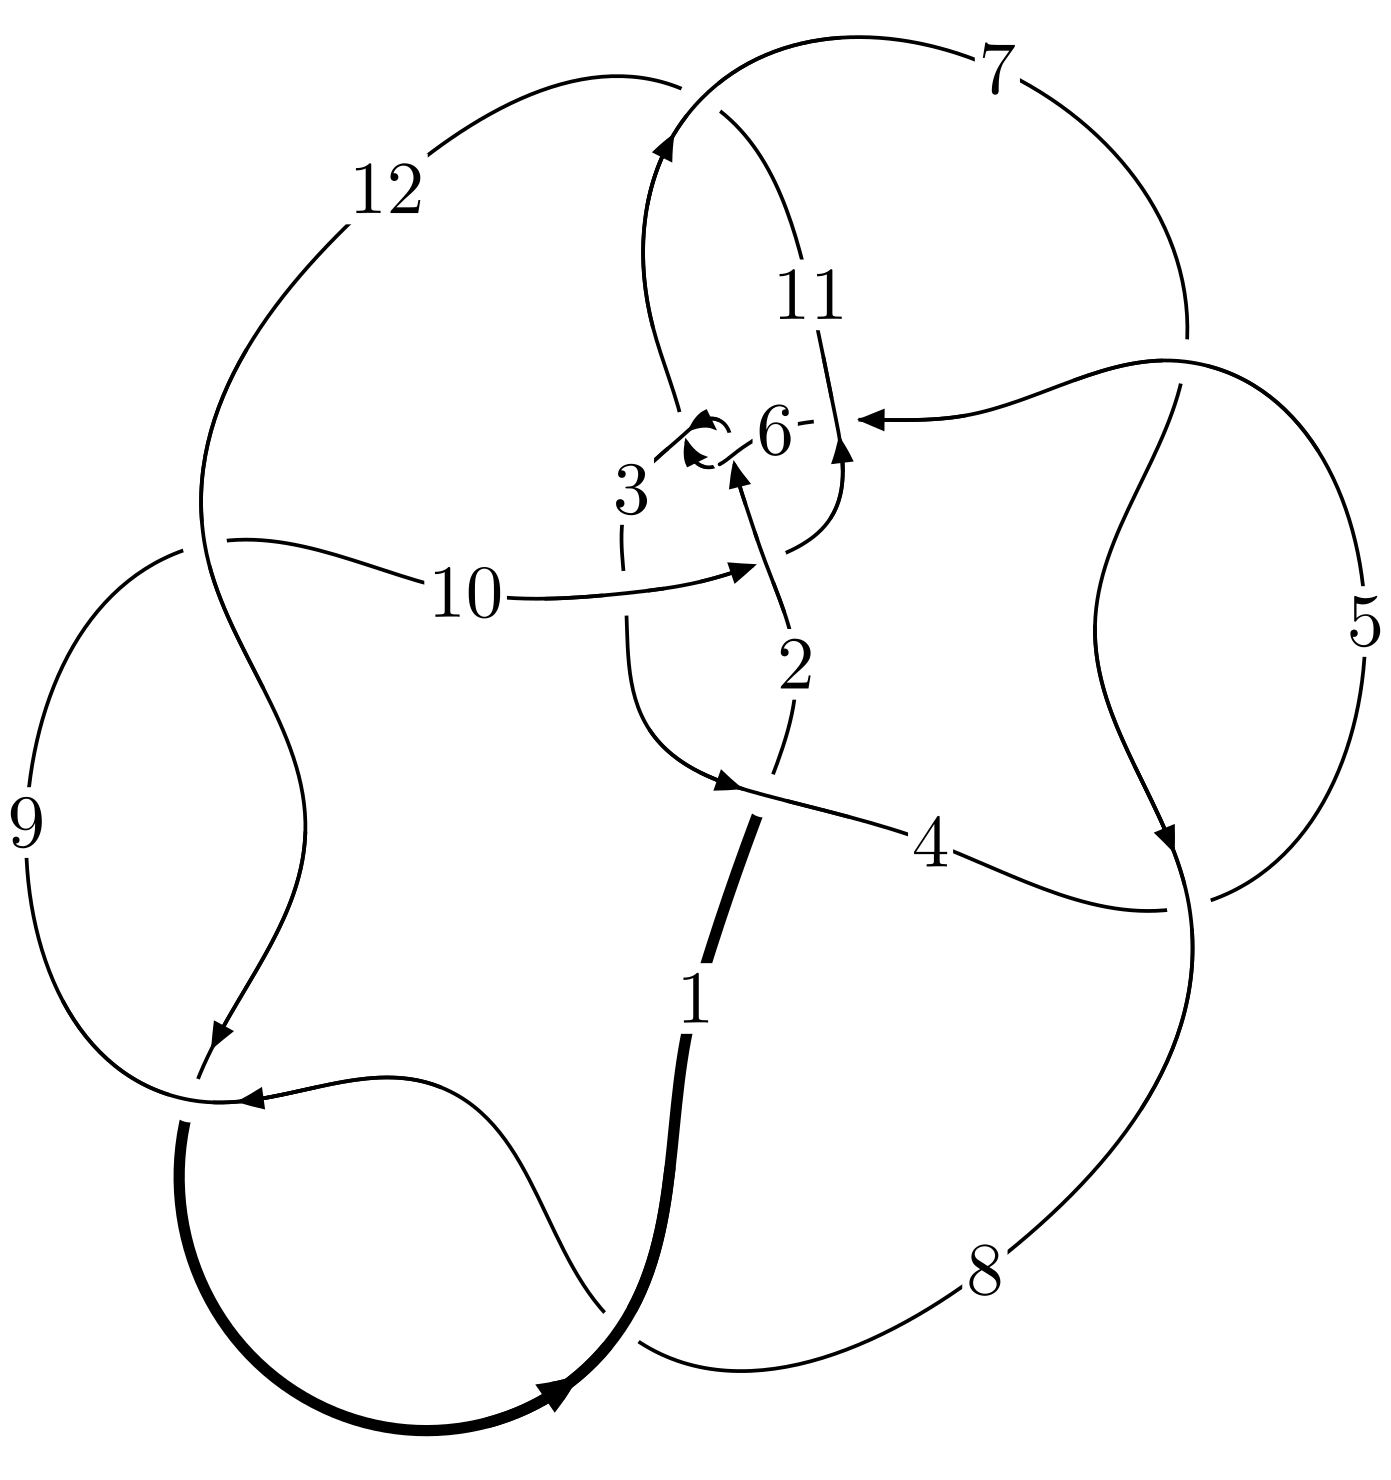
\includegraphics[width=112pt]{../../../GIT/diagram.site/Diagrams/png/1751_12a_0950.png}\\
\ \ \ A knot diagram\footnotemark}&
\allowdisplaybreaks
\textbf{Linearized knot diagam} \\
\cline{2-2}
 &
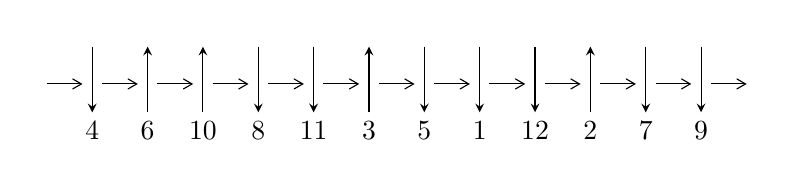
\begin{tikzpicture}[x=20pt, y=17pt]
	% nodes
	\node (C0) at (0, 0) {};
	\node (C1) at (1, 0) {};
	\node (C1U) at (1, +1) {};
	\node (C1D) at (1, -1) {4};

	\node (C2) at (2, 0) {};
	\node (C2U) at (2, +1) {};
	\node (C2D) at (2, -1) {6};

	\node (C3) at (3, 0) {};
	\node (C3U) at (3, +1) {};
	\node (C3D) at (3, -1) {10};

	\node (C4) at (4, 0) {};
	\node (C4U) at (4, +1) {};
	\node (C4D) at (4, -1) {8};

	\node (C5) at (5, 0) {};
	\node (C5U) at (5, +1) {};
	\node (C5D) at (5, -1) {11};

	\node (C6) at (6, 0) {};
	\node (C6U) at (6, +1) {};
	\node (C6D) at (6, -1) {3};

	\node (C7) at (7, 0) {};
	\node (C7U) at (7, +1) {};
	\node (C7D) at (7, -1) {5};

	\node (C8) at (8, 0) {};
	\node (C8U) at (8, +1) {};
	\node (C8D) at (8, -1) {1};

	\node (C9) at (9, 0) {};
	\node (C9U) at (9, +1) {};
	\node (C9D) at (9, -1) {12};

	\node (C10) at (10, 0) {};
	\node (C10U) at (10, +1) {};
	\node (C10D) at (10, -1) {2};

	\node (C11) at (11, 0) {};
	\node (C11U) at (11, +1) {};
	\node (C11D) at (11, -1) {7};

	\node (C12) at (12, 0) {};
	\node (C12U) at (12, +1) {};
	\node (C12D) at (12, -1) {9};
	\node (C13) at (13, 0) {};

	% arrows
	\draw[->,>={angle 60}]
	(C0) edge (C1) (C1) edge (C2) (C2) edge (C3) (C3) edge (C4) (C4) edge (C5) (C5) edge (C6) (C6) edge (C7) (C7) edge (C8) (C8) edge (C9) (C9) edge (C10) (C10) edge (C11) (C11) edge (C12) (C12) edge (C13) ;	\draw[->,>=stealth]
	(C1U) edge (C1D) (C2D) edge (C2U) (C3D) edge (C3U) (C4U) edge (C4D) (C5U) edge (C5D) (C6D) edge (C6U) (C7U) edge (C7D) (C8U) edge (C8D) (C9U) edge (C9D) (C10D) edge (C10U) (C11U) edge (C11D) (C12U) edge (C12D) ;
	\end{tikzpicture} \\
\hhline{~~} \\& 
\textbf{Solving Sequence} \\ \cline{2-2} 
 &
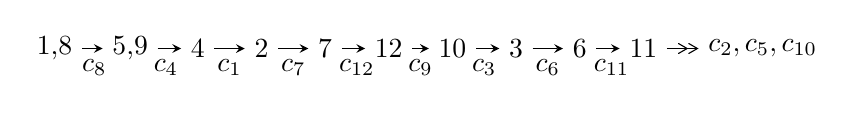
\begin{tikzpicture}[x=23pt, y=7pt]
	% node
	\node (A0) at (-1/8, 0) {1,8};
	\node (A1) at (17/16, 0) {5,9};
	\node (A2) at (17/8, 0) {4};
	\node (A3) at (25/8, 0) {2};
	\node (A4) at (33/8, 0) {7};
	\node (A5) at (41/8, 0) {12};
	\node (A6) at (49/8, 0) {10};
	\node (A7) at (57/8, 0) {3};
	\node (A8) at (65/8, 0) {6};
	\node (A9) at (73/8, 0) {11};
	\node (C1) at (1/2, -1) {$c_{8}$};
	\node (C2) at (13/8, -1) {$c_{4}$};
	\node (C3) at (21/8, -1) {$c_{1}$};
	\node (C4) at (29/8, -1) {$c_{7}$};
	\node (C5) at (37/8, -1) {$c_{12}$};
	\node (C6) at (45/8, -1) {$c_{9}$};
	\node (C7) at (53/8, -1) {$c_{3}$};
	\node (C8) at (61/8, -1) {$c_{6}$};
	\node (C9) at (69/8, -1) {$c_{11}$};
	\node (A10) at (11, 0) {$c_{2},c_{5},c_{10}$};

	% edge
	\draw[->,>=stealth]	
	(A0) edge (A1) (A1) edge (A2) (A2) edge (A3) (A3) edge (A4) (A4) edge (A5) (A5) edge (A6) (A6) edge (A7) (A7) edge (A8) (A8) edge (A9) ;
	\draw[->>,>={angle 60}]	
	(A9) edge (A10);
\end{tikzpicture} \\ 

\end{tabular} \\

\footnotetext{
The image of knot diagram is generated by the software ``\textbf{Draw programme}" developed by Andrew Bartholomew(\url{http://www.layer8.co.uk/maths/draw/index.htm\#Running-draw}), where we modified some parts for our purpose(\url{https://github.com/CATsTAILs/LinksPainter}).
}\phantom \\ \newline 
\centering \textbf{Ideals for irreducible components\footnotemark of $X_{\text{par}}$} 
 
\begin{align*}
I^u_{1}&=\langle 
3.22224\times10^{411} u^{131}+1.29708\times10^{411} u^{130}+\cdots+4.45032\times10^{412} b+8.97585\times10^{412},\\
\phantom{I^u_{1}}&\phantom{= \langle  }3.48045\times10^{415} u^{131}-1.50529\times10^{416} u^{130}+\cdots+2.38982\times10^{415} a+3.14627\times10^{416},\\
\phantom{I^u_{1}}&\phantom{= \langle  }u^{132}-4 u^{131}+\cdots+59 u+3\rangle \\
I^u_{2}&=\langle 
305214 u^{33}-1443972 u^{32}+\cdots+1901663 b+378921,\\
\phantom{I^u_{2}}&\phantom{= \langle  }762076 u^{33}-6622618 u^{32}+\cdots+1901663 a+2163731,\;u^{34}-9 u^{33}+\cdots-2 u+1\rangle \\
\\
\end{align*}
\raggedright * 2 irreducible components of $\dim_{\mathbb{C}}=0$, with total 166 representations.\\
\footnotetext{All coefficients of polynomials are rational numbers. But the coefficients are sometimes approximated in decimal forms when there is not enough margin.}
\newpage
\renewcommand{\arraystretch}{1}
\centering \section*{I. $I^u_{1}= \langle 3.22\times10^{411} u^{131}+1.30\times10^{411} u^{130}+\cdots+4.45\times10^{412} b+8.98\times10^{412},\;3.48\times10^{415} u^{131}-1.51\times10^{416} u^{130}+\cdots+2.39\times10^{415} a+3.15\times10^{416},\;u^{132}-4 u^{131}+\cdots+59 u+3 \rangle$}
\flushleft \textbf{(i) Arc colorings}\\
\begin{tabular}{m{7pt} m{180pt} m{7pt} m{180pt} }
\flushright $a_{1}=$&$\begin{pmatrix}0\\u\end{pmatrix}$ \\
\flushright $a_{8}=$&$\begin{pmatrix}1\\0\end{pmatrix}$ \\
\flushright $a_{5}=$&$\begin{pmatrix}-1.45636 u^{131}+6.29873 u^{130}+\cdots-186.709 u-13.1653\\-0.0724047 u^{131}-0.0291458 u^{130}+\cdots-38.1921 u-2.01690\end{pmatrix}$ \\
\flushright $a_{9}=$&$\begin{pmatrix}1\\u^2\end{pmatrix}$ \\
\flushright $a_{4}=$&$\begin{pmatrix}-1.52877 u^{131}+6.26959 u^{130}+\cdots-224.901 u-15.1822\\-0.0724047 u^{131}-0.0291458 u^{130}+\cdots-38.1921 u-2.01690\end{pmatrix}$ \\
\flushright $a_{2}=$&$\begin{pmatrix}2.37691 u^{131}-9.29606 u^{130}+\cdots+880.320 u+56.1784\\0.0809590 u^{131}-0.820963 u^{130}+\cdots-1.44871 u+0.631557\end{pmatrix}$ \\
\flushright $a_{7}=$&$\begin{pmatrix}-0.915943 u^{131}+3.04478 u^{130}+\cdots-224.443 u-14.1366\\0.705423 u^{131}-2.12174 u^{130}+\cdots+5.02828 u+0.267268\end{pmatrix}$ \\
\flushright $a_{12}=$&$\begin{pmatrix}u\\u^3+u\end{pmatrix}$ \\
\flushright $a_{10}=$&$\begin{pmatrix}u^2+1\\u^4+2 u^2\end{pmatrix}$ \\
\flushright $a_{3}=$&$\begin{pmatrix}-1.66495 u^{131}+7.41381 u^{130}+\cdots-222.553 u-15.4836\\-0.0541848 u^{131}-0.286281 u^{130}+\cdots-44.0633 u-2.32385\end{pmatrix}$ \\
\flushright $a_{6}=$&$\begin{pmatrix}-1.19945 u^{131}+5.10715 u^{130}+\cdots-725.676 u-44.0069\\0.000210381 u^{131}-0.330833 u^{130}+\cdots-29.0630 u-3.13429\end{pmatrix}$ \\
\flushright $a_{11}=$&$\begin{pmatrix}5.31674 u^{131}-22.2442 u^{130}+\cdots+939.143 u+46.8844\\0.111780 u^{131}+0.127260 u^{130}+\cdots+152.646 u+9.58358\end{pmatrix}$\\&\end{tabular}
\flushleft \textbf{(ii) Obstruction class $= -1$}\\~\\
\flushleft \textbf{(iii) Cusp Shapes $= -0.631647 u^{131}+2.56905 u^{130}+\cdots-968.511 u-71.1945$}\\~\\
\newpage\renewcommand{\arraystretch}{1}
\flushleft \textbf{(iv) u-Polynomials at the component}\newline \\
\begin{tabular}{m{50pt}|m{274pt}}
Crossings & \hspace{64pt}u-Polynomials at each crossing \\
\hline $$\begin{aligned}c_{1}\end{aligned}$$&$\begin{aligned}
&u^{132}-12 u^{131}+\cdots-2438849515 u+240939553
\end{aligned}$\\
\hline $$\begin{aligned}c_{2},c_{6}\end{aligned}$$&$\begin{aligned}
&u^{132}-4 u^{131}+\cdots-530 u+259
\end{aligned}$\\
\hline $$\begin{aligned}c_{3}\end{aligned}$$&$\begin{aligned}
&u^{132}+u^{131}+\cdots+69461 u-1783
\end{aligned}$\\
\hline $$\begin{aligned}c_{4},c_{7}\end{aligned}$$&$\begin{aligned}
&u^{132}-8 u^{131}+\cdots-2101 u+581
\end{aligned}$\\
\hline $$\begin{aligned}c_{5}\end{aligned}$$&$\begin{aligned}
&u^{132}+u^{131}+\cdots+1631088 u+611587
\end{aligned}$\\
\hline $$\begin{aligned}c_{8},c_{9},c_{12}\end{aligned}$$&$\begin{aligned}
&u^{132}+4 u^{131}+\cdots-59 u+3
\end{aligned}$\\
\hline $$\begin{aligned}c_{10}\end{aligned}$$&$\begin{aligned}
&u^{132}-15 u^{130}+\cdots+7439 u+1091
\end{aligned}$\\
\hline $$\begin{aligned}c_{11}\end{aligned}$$&$\begin{aligned}
&u^{132}+u^{131}+\cdots+7866797 u+1297931
\end{aligned}$\\
\hline
\end{tabular}\\~\\
\newpage\renewcommand{\arraystretch}{1}
\flushleft \textbf{(v) Riley Polynomials at the component}\newline \\
\begin{tabular}{m{50pt}|m{274pt}}
Crossings & \hspace{64pt}Riley Polynomials at each crossing \\
\hline $$\begin{aligned}c_{1}\end{aligned}$$&$\begin{aligned}
&y^{132}+60 y^{131}+\cdots+887267153635262571 y+58051868199839809
\end{aligned}$\\
\hline $$\begin{aligned}c_{2},c_{6}\end{aligned}$$&$\begin{aligned}
&y^{132}-82 y^{131}+\cdots-3272868 y+67081
\end{aligned}$\\
\hline $$\begin{aligned}c_{3}\end{aligned}$$&$\begin{aligned}
&y^{132}-11 y^{131}+\cdots-8154857603 y+3179089
\end{aligned}$\\
\hline $$\begin{aligned}c_{4},c_{7}\end{aligned}$$&$\begin{aligned}
&y^{132}+118 y^{131}+\cdots+81012553 y+337561
\end{aligned}$\\
\hline $$\begin{aligned}c_{5}\end{aligned}$$&$\begin{aligned}
&y^{132}+39 y^{131}+\cdots+21589787450618 y+374038658569
\end{aligned}$\\
\hline $$\begin{aligned}c_{8},c_{9},c_{12}\end{aligned}$$&$\begin{aligned}
&y^{132}+136 y^{131}+\cdots+245 y+9
\end{aligned}$\\
\hline $$\begin{aligned}c_{10}\end{aligned}$$&$\begin{aligned}
&y^{132}-30 y^{131}+\cdots-203221589 y+1190281
\end{aligned}$\\
\hline $$\begin{aligned}c_{11}\end{aligned}$$&$\begin{aligned}
&y^{132}+51 y^{131}+\cdots+56520089925371 y+1684624880761
\end{aligned}$\\
\hline
\end{tabular}\\~\\
\newpage\flushleft \textbf{(vi) Complex Volumes and Cusp Shapes}
$$\begin{array}{c|c|c}  
\text{Solutions to }I^u_{1}& \I (\text{vol} + \sqrt{-1}CS) & \text{Cusp shape}\\
 \hline 
\begin{aligned}
u &= -0.767053 + 0.620115 I \\
a &= \phantom{-}0.736005 + 0.407715 I \\
b &= -0.190482 - 1.331180 I\end{aligned}
 & \phantom{-}4.08639 - 3.30659 I & \phantom{-0.000000 } 0 \\ \hline\begin{aligned}
u &= -0.767053 - 0.620115 I \\
a &= \phantom{-}0.736005 - 0.407715 I \\
b &= -0.190482 + 1.331180 I\end{aligned}
 & \phantom{-}4.08639 + 3.30659 I & \phantom{-0.000000 } 0 \\ \hline\begin{aligned}
u &= \phantom{-}0.114709 + 1.029170 I \\
a &= \phantom{-}0.536516 - 0.677578 I \\
b &= \phantom{-}0.475424 + 1.166190 I\end{aligned}
 & \phantom{-}6.99783 - 6.24714 I & \phantom{-0.000000 } 0 \\ \hline\begin{aligned}
u &= \phantom{-}0.114709 - 1.029170 I \\
a &= \phantom{-}0.536516 + 0.677578 I \\
b &= \phantom{-}0.475424 - 1.166190 I\end{aligned}
 & \phantom{-}6.99783 + 6.24714 I & \phantom{-0.000000 } 0 \\ \hline\begin{aligned}
u &= -0.807298 + 0.525025 I \\
a &= -0.894899 - 0.633983 I \\
b &= -0.40014 + 1.42345 I\end{aligned}
 & \phantom{-}3.81199 + 8.60180 I & \phantom{-0.000000 } 0 \\ \hline\begin{aligned}
u &= -0.807298 - 0.525025 I \\
a &= -0.894899 + 0.633983 I \\
b &= -0.40014 - 1.42345 I\end{aligned}
 & \phantom{-}3.81199 - 8.60180 I & \phantom{-0.000000 } 0 \\ \hline\begin{aligned}
u &= -0.893205 + 0.594651 I \\
a &= \phantom{-}0.775847 + 0.746866 I \\
b &= \phantom{-}0.39069 - 1.42500 I\end{aligned}
 & \phantom{-}7.4643 + 14.2993 I & \phantom{-0.000000 } 0 \\ \hline\begin{aligned}
u &= -0.893205 - 0.594651 I \\
a &= \phantom{-}0.775847 - 0.746866 I \\
b &= \phantom{-}0.39069 + 1.42500 I\end{aligned}
 & \phantom{-}7.4643 - 14.2993 I & \phantom{-0.000000 } 0 \\ \hline\begin{aligned}
u &= \phantom{-}0.923755 + 0.556913 I \\
a &= -0.418791 + 0.832376 I \\
b &= -0.120619 - 1.302090 I\end{aligned}
 & \phantom{-}2.71743 - 2.20489 I & \phantom{-0.000000 } 0 \\ \hline\begin{aligned}
u &= \phantom{-}0.923755 - 0.556913 I \\
a &= -0.418791 - 0.832376 I \\
b &= -0.120619 + 1.302090 I\end{aligned}
 & \phantom{-}2.71743 + 2.20489 I & \phantom{-0.000000 } 0\\
 \hline 
 \end{array}$$\newpage$$\begin{array}{c|c|c}  
\text{Solutions to }I^u_{1}& \I (\text{vol} + \sqrt{-1}CS) & \text{Cusp shape}\\
 \hline 
\begin{aligned}
u &= \phantom{-}0.499948 + 0.985294 I \\
a &= -0.200595 + 0.653013 I \\
b &= -0.302170 - 0.383862 I\end{aligned}
 & \phantom{-}1.54660 - 4.25235 I & \phantom{-0.000000 } 0 \\ \hline\begin{aligned}
u &= \phantom{-}0.499948 - 0.985294 I \\
a &= -0.200595 - 0.653013 I \\
b &= -0.302170 + 0.383862 I\end{aligned}
 & \phantom{-}1.54660 + 4.25235 I & \phantom{-0.000000 } 0 \\ \hline\begin{aligned}
u &= \phantom{-}0.979892 + 0.525077 I \\
a &= \phantom{-}0.623155 - 0.398725 I \\
b &= \phantom{-}0.084096 + 1.172410 I\end{aligned}
 & \phantom{-}2.15340 - 2.11704 I & \phantom{-0.000000 } 0 \\ \hline\begin{aligned}
u &= \phantom{-}0.979892 - 0.525077 I \\
a &= \phantom{-}0.623155 + 0.398725 I \\
b &= \phantom{-}0.084096 - 1.172410 I\end{aligned}
 & \phantom{-}2.15340 + 2.11704 I & \phantom{-0.000000 } 0 \\ \hline\begin{aligned}
u &= \phantom{-}0.819959 + 0.296432 I \\
a &= \phantom{-}0.818801 + 0.182317 I \\
b &= \phantom{-}0.027202 + 1.177160 I\end{aligned}
 & \phantom{-}2.37328 - 1.93366 I & \phantom{-0.000000 } 0 \\ \hline\begin{aligned}
u &= \phantom{-}0.819959 - 0.296432 I \\
a &= \phantom{-}0.818801 - 0.182317 I \\
b &= \phantom{-}0.027202 - 1.177160 I\end{aligned}
 & \phantom{-}2.37328 + 1.93366 I & \phantom{-0.000000 } 0 \\ \hline\begin{aligned}
u &= -0.813878 + 0.310335 I \\
a &= -0.458140 - 0.080231 I \\
b &= \phantom{-}0.161876 + 1.393950 I\end{aligned}
 & \phantom{-}7.85556 + 0.90527 I & \phantom{-0.000000 } 0 \\ \hline\begin{aligned}
u &= -0.813878 - 0.310335 I \\
a &= -0.458140 + 0.080231 I \\
b &= \phantom{-}0.161876 - 1.393950 I\end{aligned}
 & \phantom{-}7.85556 - 0.90527 I & \phantom{-0.000000 } 0 \\ \hline\begin{aligned}
u &= \phantom{-}0.316942 + 0.805933 I \\
a &= \phantom{-}0.272424 + 1.279480 I \\
b &= -0.195749 - 0.795398 I\end{aligned}
 & \phantom{-}1.46726 - 1.82664 I & \phantom{-0.000000 } 0 \\ \hline\begin{aligned}
u &= \phantom{-}0.316942 - 0.805933 I \\
a &= \phantom{-}0.272424 - 1.279480 I \\
b &= -0.195749 + 0.795398 I\end{aligned}
 & \phantom{-}1.46726 + 1.82664 I & \phantom{-0.000000 } 0\\
 \hline 
 \end{array}$$\newpage$$\begin{array}{c|c|c}  
\text{Solutions to }I^u_{1}& \I (\text{vol} + \sqrt{-1}CS) & \text{Cusp shape}\\
 \hline 
\begin{aligned}
u &= -0.616809 + 0.597964 I \\
a &= \phantom{-}1.21895 + 0.79785 I \\
b &= \phantom{-}0.38316 - 1.39154 I\end{aligned}
 & \phantom{-}8.85004 + 3.62228 I & \phantom{-0.000000 } 0 \\ \hline\begin{aligned}
u &= -0.616809 - 0.597964 I \\
a &= \phantom{-}1.21895 - 0.79785 I \\
b &= \phantom{-}0.38316 + 1.39154 I\end{aligned}
 & \phantom{-}8.85004 - 3.62228 I & \phantom{-0.000000 } 0 \\ \hline\begin{aligned}
u &= -0.942236 + 0.662943 I \\
a &= -0.588488 - 0.511150 I \\
b &= \phantom{-}0.207282 + 1.345090 I\end{aligned}
 & \phantom{-}7.55939 - 8.22426 I & \phantom{-0.000000 } 0 \\ \hline\begin{aligned}
u &= -0.942236 - 0.662943 I \\
a &= -0.588488 + 0.511150 I \\
b &= \phantom{-}0.207282 - 1.345090 I\end{aligned}
 & \phantom{-}7.55939 + 8.22426 I & \phantom{-0.000000 } 0 \\ \hline\begin{aligned}
u &= \phantom{-}0.031223 + 0.839282 I \\
a &= \phantom{-}0.750922 - 1.145570 I \\
b &= -0.265590 + 0.187892 I\end{aligned}
 & -0.216709 - 1.247950 I & \phantom{-0.000000 } 0 \\ \hline\begin{aligned}
u &= \phantom{-}0.031223 - 0.839282 I \\
a &= \phantom{-}0.750922 + 1.145570 I \\
b &= -0.265590 - 0.187892 I\end{aligned}
 & -0.216709 + 1.247950 I & \phantom{-0.000000 } 0 \\ \hline\begin{aligned}
u &= \phantom{-}0.504286 + 1.065090 I \\
a &= \phantom{-}0.070744 - 1.396820 I \\
b &= \phantom{-}0.052137 + 0.853579 I\end{aligned}
 & \phantom{-}2.68256 - 3.49929 I & \phantom{-0.000000 } 0 \\ \hline\begin{aligned}
u &= \phantom{-}0.504286 - 1.065090 I \\
a &= \phantom{-}0.070744 + 1.396820 I \\
b &= \phantom{-}0.052137 - 0.853579 I\end{aligned}
 & \phantom{-}2.68256 + 3.49929 I & \phantom{-0.000000 } 0 \\ \hline\begin{aligned}
u &= \phantom{-}0.696281 + 0.431174 I \\
a &= \phantom{-}0.339990 - 0.113857 I \\
b &= \phantom{-}0.413409 + 0.047062 I\end{aligned}
 & -0.60011 - 2.20926 I & \phantom{-0.000000 } 0 \\ \hline\begin{aligned}
u &= \phantom{-}0.696281 - 0.431174 I \\
a &= \phantom{-}0.339990 + 0.113857 I \\
b &= \phantom{-}0.413409 - 0.047062 I\end{aligned}
 & -0.60011 + 2.20926 I & \phantom{-0.000000 } 0\\
 \hline 
 \end{array}$$\newpage$$\begin{array}{c|c|c}  
\text{Solutions to }I^u_{1}& \I (\text{vol} + \sqrt{-1}CS) & \text{Cusp shape}\\
 \hline 
\begin{aligned}
u &= \phantom{-}0.919366 + 0.754060 I \\
a &= \phantom{-}0.638803 - 1.054440 I \\
b &= \phantom{-}0.098187 + 1.275980 I\end{aligned}
 & \phantom{-}3.31816 - 4.14785 I & \phantom{-0.000000 } 0 \\ \hline\begin{aligned}
u &= \phantom{-}0.919366 - 0.754060 I \\
a &= \phantom{-}0.638803 + 1.054440 I \\
b &= \phantom{-}0.098187 - 1.275980 I\end{aligned}
 & \phantom{-}3.31816 + 4.14785 I & \phantom{-0.000000 } 0 \\ \hline\begin{aligned}
u &= \phantom{-}0.289926 + 1.164690 I \\
a &= \phantom{-}0.725260 - 0.707252 I \\
b &= \phantom{-}0.367811 + 1.161470 I\end{aligned}
 & \phantom{-}6.96025 - 6.23487 I & \phantom{-0.000000 } 0 \\ \hline\begin{aligned}
u &= \phantom{-}0.289926 - 1.164690 I \\
a &= \phantom{-}0.725260 + 0.707252 I \\
b &= \phantom{-}0.367811 - 1.161470 I\end{aligned}
 & \phantom{-}6.96025 + 6.23487 I & \phantom{-0.000000 } 0 \\ \hline\begin{aligned}
u &= -0.431488 + 0.653862 I \\
a &= -0.50887 + 1.33602 I \\
b &= \phantom{-}0.444064 + 0.080062 I\end{aligned}
 & \phantom{-}2.95782 - 5.69512 I & \phantom{-0.000000 } 0 \\ \hline\begin{aligned}
u &= -0.431488 - 0.653862 I \\
a &= -0.50887 - 1.33602 I \\
b &= \phantom{-}0.444064 - 0.080062 I\end{aligned}
 & \phantom{-}2.95782 + 5.69512 I & \phantom{-0.000000 } 0 \\ \hline\begin{aligned}
u &= -0.083243 + 1.230380 I \\
a &= \phantom{-}0.479669 - 0.431619 I \\
b &= -0.455547 - 0.763476 I\end{aligned}
 & \phantom{-}2.81507 - 0.60865 I & \phantom{-0.000000 } 0 \\ \hline\begin{aligned}
u &= -0.083243 - 1.230380 I \\
a &= \phantom{-}0.479669 + 0.431619 I \\
b &= -0.455547 + 0.763476 I\end{aligned}
 & \phantom{-}2.81507 + 0.60865 I & \phantom{-0.000000 } 0 \\ \hline\begin{aligned}
u &= \phantom{-}0.381803 + 0.664483 I \\
a &= -2.06953 + 1.64664 I \\
b &= \phantom{-}0.032513 - 1.278260 I\end{aligned}
 & \phantom{-}6.92478 - 4.41301 I & \phantom{-0.000000 } 0 \\ \hline\begin{aligned}
u &= \phantom{-}0.381803 - 0.664483 I \\
a &= -2.06953 - 1.64664 I \\
b &= \phantom{-}0.032513 + 1.278260 I\end{aligned}
 & \phantom{-}6.92478 + 4.41301 I & \phantom{-0.000000 } 0\\
 \hline 
 \end{array}$$\newpage$$\begin{array}{c|c|c}  
\text{Solutions to }I^u_{1}& \I (\text{vol} + \sqrt{-1}CS) & \text{Cusp shape}\\
 \hline 
\begin{aligned}
u &= \phantom{-}0.553514 + 0.518230 I \\
a &= -0.489696 + 0.584603 I \\
b &= -0.250986 - 1.384720 I\end{aligned}
 & \phantom{-}3.26652 - 2.51546 I & \phantom{-0.000000 } 0 \\ \hline\begin{aligned}
u &= \phantom{-}0.553514 - 0.518230 I \\
a &= -0.489696 - 0.584603 I \\
b &= -0.250986 + 1.384720 I\end{aligned}
 & \phantom{-}3.26652 + 2.51546 I & \phantom{-0.000000 } 0 \\ \hline\begin{aligned}
u &= \phantom{-}0.986647 + 0.790916 I \\
a &= -0.476862 + 0.636183 I \\
b &= -0.175316 - 1.165180 I\end{aligned}
 & \phantom{-}2.91018 - 4.54846 I & \phantom{-0.000000 } 0 \\ \hline\begin{aligned}
u &= \phantom{-}0.986647 - 0.790916 I \\
a &= -0.476862 - 0.636183 I \\
b &= -0.175316 + 1.165180 I\end{aligned}
 & \phantom{-}2.91018 + 4.54846 I & \phantom{-0.000000 } 0 \\ \hline\begin{aligned}
u &= -0.606905 + 0.403437 I \\
a &= \phantom{-}0.546328 - 0.083019 I \\
b &= \phantom{-}0.988181 - 0.235108 I\end{aligned}
 & \phantom{-}2.19288 + 9.43541 I & \phantom{-0.000000 } 0 \\ \hline\begin{aligned}
u &= -0.606905 - 0.403437 I \\
a &= \phantom{-}0.546328 + 0.083019 I \\
b &= \phantom{-}0.988181 + 0.235108 I\end{aligned}
 & \phantom{-}2.19288 - 9.43541 I & \phantom{-0.000000 } 0 \\ \hline\begin{aligned}
u &= \phantom{-}0.563761 + 0.423889 I \\
a &= -0.229371 - 0.862700 I \\
b &= -0.612479 + 0.363883 I\end{aligned}
 & \phantom{-}0.61224 - 1.56921 I & \phantom{-0.000000 } 0 \\ \hline\begin{aligned}
u &= \phantom{-}0.563761 - 0.423889 I \\
a &= -0.229371 + 0.862700 I \\
b &= -0.612479 - 0.363883 I\end{aligned}
 & \phantom{-}0.61224 + 1.56921 I & \phantom{-0.000000 } 0 \\ \hline\begin{aligned}
u &= \phantom{-}0.704423\phantom{ +0.000000I} \\
a &= -0.123732\phantom{ +0.000000I} \\
b &= -0.517903\phantom{ +0.000000I}\end{aligned}
 & -1.19742\phantom{ +0.000000I} & \phantom{-0.000000 } 0 \\ \hline\begin{aligned}
u &= -0.192255 + 1.334470 I \\
a &= -0.773697 + 0.750231 I \\
b &= \phantom{-}0.307385 + 0.384534 I\end{aligned}
 & \phantom{-}6.77695 + 6.18958 I & \phantom{-0.000000 } 0\\
 \hline 
 \end{array}$$\newpage$$\begin{array}{c|c|c}  
\text{Solutions to }I^u_{1}& \I (\text{vol} + \sqrt{-1}CS) & \text{Cusp shape}\\
 \hline 
\begin{aligned}
u &= -0.192255 - 1.334470 I \\
a &= -0.773697 - 0.750231 I \\
b &= \phantom{-}0.307385 - 0.384534 I\end{aligned}
 & \phantom{-}6.77695 - 6.18958 I & \phantom{-0.000000 } 0 \\ \hline\begin{aligned}
u &= \phantom{-}0.016225 + 1.364930 I \\
a &= \phantom{-}0.414013 + 0.458130 I \\
b &= \phantom{-}0.680119 - 0.431337 I\end{aligned}
 & \phantom{-}5.04727 - 2.24596 I & \phantom{-0.000000 } 0 \\ \hline\begin{aligned}
u &= \phantom{-}0.016225 - 1.364930 I \\
a &= \phantom{-}0.414013 - 0.458130 I \\
b &= \phantom{-}0.680119 + 0.431337 I\end{aligned}
 & \phantom{-}5.04727 + 2.24596 I & \phantom{-0.000000 } 0 \\ \hline\begin{aligned}
u &= \phantom{-}0.089681 + 1.372730 I \\
a &= \phantom{-}0.341213 + 0.455127 I \\
b &= -0.918176 - 0.511825 I\end{aligned}
 & \phantom{-}3.10244 - 2.09594 I & \phantom{-0.000000 } 0 \\ \hline\begin{aligned}
u &= \phantom{-}0.089681 - 1.372730 I \\
a &= \phantom{-}0.341213 - 0.455127 I \\
b &= -0.918176 + 0.511825 I\end{aligned}
 & \phantom{-}3.10244 + 2.09594 I & \phantom{-0.000000 } 0 \\ \hline\begin{aligned}
u &= \phantom{-}0.592474 + 0.174546 I \\
a &= \phantom{-}0.543867 + 1.128330 I \\
b &= \phantom{-}0.402756 - 0.457035 I\end{aligned}
 & \phantom{-}0.152820 - 0.389619 I & -4.00000 - 2.43878 I \\ \hline\begin{aligned}
u &= \phantom{-}0.592474 - 0.174546 I \\
a &= \phantom{-}0.543867 - 1.128330 I \\
b &= \phantom{-}0.402756 + 0.457035 I\end{aligned}
 & \phantom{-}0.152820 + 0.389619 I & -4.00000 + 2.43878 I \\ \hline\begin{aligned}
u &= -0.105077 + 1.405480 I \\
a &= -0.55139 - 1.42451 I \\
b &= -0.766764 + 0.978278 I\end{aligned}
 & \phantom{-}4.43357 + 3.99471 I & \phantom{-0.000000 } 0 \\ \hline\begin{aligned}
u &= -0.105077 - 1.405480 I \\
a &= -0.55139 + 1.42451 I \\
b &= -0.766764 - 0.978278 I\end{aligned}
 & \phantom{-}4.43357 - 3.99471 I & \phantom{-0.000000 } 0 \\ \hline\begin{aligned}
u &= -0.102146 + 1.408590 I \\
a &= \phantom{-}0.80774 + 1.89483 I \\
b &= \phantom{-}0.24261 - 1.46987 I\end{aligned}
 & \phantom{-}10.91370 + 0.95614 I & \phantom{-0.000000 } 0\\
 \hline 
 \end{array}$$\newpage$$\begin{array}{c|c|c}  
\text{Solutions to }I^u_{1}& \I (\text{vol} + \sqrt{-1}CS) & \text{Cusp shape}\\
 \hline 
\begin{aligned}
u &= -0.102146 - 1.408590 I \\
a &= \phantom{-}0.80774 - 1.89483 I \\
b &= \phantom{-}0.24261 + 1.46987 I\end{aligned}
 & \phantom{-}10.91370 - 0.95614 I & \phantom{-0.000000 } 0 \\ \hline\begin{aligned}
u &= \phantom{-}0.232214 + 0.537737 I \\
a &= \phantom{-}0.58070 + 1.70480 I \\
b &= -0.142325 - 0.812802 I\end{aligned}
 & \phantom{-}1.40465 - 1.74138 I & \phantom{-0.000000 -}0. + 4.28223 I \\ \hline\begin{aligned}
u &= \phantom{-}0.232214 - 0.537737 I \\
a &= \phantom{-}0.58070 - 1.70480 I \\
b &= -0.142325 + 0.812802 I\end{aligned}
 & \phantom{-}1.40465 + 1.74138 I & \phantom{-0.000000 } 0. - 4.28223 I \\ \hline\begin{aligned}
u &= -0.491845 + 0.309179 I \\
a &= -0.832695 + 0.027029 I \\
b &= -1.024750 + 0.253442 I\end{aligned}
 & -1.46863 + 3.62459 I & -5.39704 - 10.50305 I \\ \hline\begin{aligned}
u &= -0.491845 - 0.309179 I \\
a &= -0.832695 - 0.027029 I \\
b &= -1.024750 - 0.253442 I\end{aligned}
 & -1.46863 - 3.62459 I & -5.39704 + 10.50305 I \\ \hline\begin{aligned}
u &= -0.201896 + 0.536883 I \\
a &= \phantom{-}0.505022 + 0.578194 I \\
b &= \phantom{-}0.951214 - 0.203933 I\end{aligned}
 & \phantom{-}3.80422 - 1.02783 I & \phantom{-}3.93619 - 2.26152 I \\ \hline\begin{aligned}
u &= -0.201896 - 0.536883 I \\
a &= \phantom{-}0.505022 - 0.578194 I \\
b &= \phantom{-}0.951214 + 0.203933 I\end{aligned}
 & \phantom{-}3.80422 + 1.02783 I & \phantom{-}3.93619 + 2.26152 I \\ \hline\begin{aligned}
u &= \phantom{-}0.570323\phantom{ +0.000000I} \\
a &= -0.0425588\phantom{ +0.000000I} \\
b &= -0.537302\phantom{ +0.000000I}\end{aligned}
 & -1.23428\phantom{ +0.000000I} & -9.88860\phantom{ +0.000000I} \\ \hline\begin{aligned}
u &= -0.01841 + 1.43051 I \\
a &= -0.05454 - 2.65151 I \\
b &= -0.227464 + 1.251790 I\end{aligned}
 & \phantom{-}4.71659 + 2.32241 I & \phantom{-0.000000 } 0 \\ \hline\begin{aligned}
u &= -0.01841 - 1.43051 I \\
a &= -0.05454 + 2.65151 I \\
b &= -0.227464 - 1.251790 I\end{aligned}
 & \phantom{-}4.71659 - 2.32241 I & \phantom{-0.000000 } 0\\
 \hline 
 \end{array}$$\newpage$$\begin{array}{c|c|c}  
\text{Solutions to }I^u_{1}& \I (\text{vol} + \sqrt{-1}CS) & \text{Cusp shape}\\
 \hline 
\begin{aligned}
u &= -0.548096 + 0.138812 I \\
a &= \phantom{-}0.53031 + 1.46961 I \\
b &= \phantom{-}0.619681 + 0.342541 I\end{aligned}
 & \phantom{-}2.19632 + 3.49075 I & -4.08845 - 5.43017 I \\ \hline\begin{aligned}
u &= -0.548096 - 0.138812 I \\
a &= \phantom{-}0.53031 - 1.46961 I \\
b &= \phantom{-}0.619681 - 0.342541 I\end{aligned}
 & \phantom{-}2.19632 - 3.49075 I & -4.08845 + 5.43017 I \\ \hline\begin{aligned}
u &= \phantom{-}0.12767 + 1.43151 I \\
a &= \phantom{-}0.086377 + 0.171716 I \\
b &= \phantom{-}0.754964 - 0.167867 I\end{aligned}
 & \phantom{-}5.27540 - 2.64634 I & \phantom{-0.000000 } 0 \\ \hline\begin{aligned}
u &= \phantom{-}0.12767 - 1.43151 I \\
a &= \phantom{-}0.086377 - 0.171716 I \\
b &= \phantom{-}0.754964 + 0.167867 I\end{aligned}
 & \phantom{-}5.27540 + 2.64634 I & \phantom{-0.000000 } 0 \\ \hline\begin{aligned}
u &= -0.14128 + 1.44569 I \\
a &= \phantom{-}0.701685 - 0.837176 I \\
b &= -1.46294 + 0.48565 I\end{aligned}
 & \phantom{-}4.24691 + 5.84943 I & \phantom{-0.000000 } 0 \\ \hline\begin{aligned}
u &= -0.14128 - 1.44569 I \\
a &= \phantom{-}0.701685 + 0.837176 I \\
b &= -1.46294 - 0.48565 I\end{aligned}
 & \phantom{-}4.24691 - 5.84943 I & \phantom{-0.000000 } 0 \\ \hline\begin{aligned}
u &= -0.05262 + 1.45372 I \\
a &= -0.21839 + 3.13591 I \\
b &= \phantom{-}0.142886 - 1.256910 I\end{aligned}
 & \phantom{-}9.74455 + 7.86908 I & \phantom{-0.000000 } 0 \\ \hline\begin{aligned}
u &= -0.05262 - 1.45372 I \\
a &= -0.21839 - 3.13591 I \\
b &= \phantom{-}0.142886 + 1.256910 I\end{aligned}
 & \phantom{-}9.74455 - 7.86908 I & \phantom{-0.000000 } 0 \\ \hline\begin{aligned}
u &= \phantom{-}0.10173 + 1.45572 I \\
a &= -0.19231 + 2.40268 I \\
b &= -0.30741 - 2.00060 I\end{aligned}
 & \phantom{-}9.37018 - 4.70111 I & \phantom{-0.000000 } 0 \\ \hline\begin{aligned}
u &= \phantom{-}0.10173 - 1.45572 I \\
a &= -0.19231 - 2.40268 I \\
b &= -0.30741 + 2.00060 I\end{aligned}
 & \phantom{-}9.37018 + 4.70111 I & \phantom{-0.000000 } 0\\
 \hline 
 \end{array}$$\newpage$$\begin{array}{c|c|c}  
\text{Solutions to }I^u_{1}& \I (\text{vol} + \sqrt{-1}CS) & \text{Cusp shape}\\
 \hline 
\begin{aligned}
u &= \phantom{-}0.24463 + 1.45153 I \\
a &= -0.001700 - 0.405065 I \\
b &= \phantom{-}0.568880 + 0.311688 I\end{aligned}
 & \phantom{-}5.42968 - 5.64561 I & \phantom{-0.000000 } 0 \\ \hline\begin{aligned}
u &= \phantom{-}0.24463 - 1.45153 I \\
a &= -0.001700 + 0.405065 I \\
b &= \phantom{-}0.568880 - 0.311688 I\end{aligned}
 & \phantom{-}5.42968 + 5.64561 I & \phantom{-0.000000 } 0 \\ \hline\begin{aligned}
u &= -0.00920 + 1.47254 I \\
a &= -0.72969 - 2.01754 I \\
b &= -0.31042 + 1.44983 I\end{aligned}
 & \phantom{-}12.36590 + 0.35979 I & \phantom{-0.000000 } 0 \\ \hline\begin{aligned}
u &= -0.00920 - 1.47254 I \\
a &= -0.72969 + 2.01754 I \\
b &= -0.31042 - 1.44983 I\end{aligned}
 & \phantom{-}12.36590 - 0.35979 I & \phantom{-0.000000 } 0 \\ \hline\begin{aligned}
u &= -0.00853 + 1.47326 I \\
a &= -0.72056 - 2.06945 I \\
b &= \phantom{-}1.21018 + 1.92495 I\end{aligned}
 & \phantom{-}11.34740 + 3.08197 I & \phantom{-0.000000 } 0 \\ \hline\begin{aligned}
u &= -0.00853 - 1.47326 I \\
a &= -0.72056 + 2.06945 I \\
b &= \phantom{-}1.21018 - 1.92495 I\end{aligned}
 & \phantom{-}11.34740 - 3.08197 I & \phantom{-0.000000 } 0 \\ \hline\begin{aligned}
u &= \phantom{-}0.07012 + 1.48677 I \\
a &= \phantom{-}0.11412 + 2.02847 I \\
b &= \phantom{-}0.232659 - 1.212280 I\end{aligned}
 & \phantom{-}7.89248 - 2.87390 I & \phantom{-0.000000 } 0 \\ \hline\begin{aligned}
u &= \phantom{-}0.07012 - 1.48677 I \\
a &= \phantom{-}0.11412 - 2.02847 I \\
b &= \phantom{-}0.232659 + 1.212280 I\end{aligned}
 & \phantom{-}7.89248 + 2.87390 I & \phantom{-0.000000 } 0 \\ \hline\begin{aligned}
u &= -0.19062 + 1.48428 I \\
a &= -0.552082 + 0.669473 I \\
b &= \phantom{-}1.350400 - 0.403507 I\end{aligned}
 & \phantom{-}8.3754 + 12.2876 I & \phantom{-0.000000 } 0 \\ \hline\begin{aligned}
u &= -0.19062 - 1.48428 I \\
a &= -0.552082 - 0.669473 I \\
b &= \phantom{-}1.350400 + 0.403507 I\end{aligned}
 & \phantom{-}8.3754 - 12.2876 I & \phantom{-0.000000 } 0\\
 \hline 
 \end{array}$$\newpage$$\begin{array}{c|c|c}  
\text{Solutions to }I^u_{1}& \I (\text{vol} + \sqrt{-1}CS) & \text{Cusp shape}\\
 \hline 
\begin{aligned}
u &= \phantom{-}0.186009 + 0.467120 I \\
a &= \phantom{-}1.32783 - 0.67696 I \\
b &= \phantom{-}0.0050287 - 0.0876047 I\end{aligned}
 & -0.265403 - 1.341610 I & -3.65967 + 3.10597 I \\ \hline\begin{aligned}
u &= \phantom{-}0.186009 - 0.467120 I \\
a &= \phantom{-}1.32783 + 0.67696 I \\
b &= \phantom{-}0.0050287 + 0.0876047 I\end{aligned}
 & -0.265403 + 1.341610 I & -3.65967 - 3.10597 I \\ \hline\begin{aligned}
u &= -0.04164 + 1.49773 I \\
a &= -0.880711 + 0.319163 I \\
b &= \phantom{-}1.52049 - 0.10487 I\end{aligned}
 & \phantom{-}10.43450 - 0.23468 I & \phantom{-0.000000 } 0 \\ \hline\begin{aligned}
u &= -0.04164 - 1.49773 I \\
a &= -0.880711 - 0.319163 I \\
b &= \phantom{-}1.52049 + 0.10487 I\end{aligned}
 & \phantom{-}10.43450 + 0.23468 I & \phantom{-0.000000 } 0 \\ \hline\begin{aligned}
u &= \phantom{-}0.17934 + 1.50397 I \\
a &= \phantom{-}0.233739 - 0.241673 I \\
b &= -0.984405 + 0.137584 I\end{aligned}
 & \phantom{-}7.00133 - 4.24104 I & \phantom{-0.000000 } 0 \\ \hline\begin{aligned}
u &= \phantom{-}0.17934 - 1.50397 I \\
a &= \phantom{-}0.233739 + 0.241673 I \\
b &= -0.984405 - 0.137584 I\end{aligned}
 & \phantom{-}7.00133 + 4.24104 I & \phantom{-0.000000 } 0 \\ \hline\begin{aligned}
u &= -0.36063 + 1.50117 I \\
a &= -0.82927 - 1.50546 I \\
b &= -0.01242 + 1.50608 I\end{aligned}
 & \phantom{-}13.6673 + 5.3531 I & \phantom{-0.000000 } 0 \\ \hline\begin{aligned}
u &= -0.36063 - 1.50117 I \\
a &= -0.82927 + 1.50546 I \\
b &= -0.01242 - 1.50608 I\end{aligned}
 & \phantom{-}13.6673 - 5.3531 I & \phantom{-0.000000 } 0 \\ \hline\begin{aligned}
u &= \phantom{-}0.00092 + 1.54768 I \\
a &= -0.481396 + 0.260915 I \\
b &= -0.307873 + 0.116910 I\end{aligned}
 & \phantom{-}10.55720 - 4.74072 I & \phantom{-0.000000 } 0 \\ \hline\begin{aligned}
u &= \phantom{-}0.00092 - 1.54768 I \\
a &= -0.481396 - 0.260915 I \\
b &= -0.307873 - 0.116910 I\end{aligned}
 & \phantom{-}10.55720 + 4.74072 I & \phantom{-0.000000 } 0\\
 \hline 
 \end{array}$$\newpage$$\begin{array}{c|c|c}  
\text{Solutions to }I^u_{1}& \I (\text{vol} + \sqrt{-1}CS) & \text{Cusp shape}\\
 \hline 
\begin{aligned}
u &= -0.20784 + 1.53929 I \\
a &= \phantom{-}0.63155 + 1.96068 I \\
b &= \phantom{-}0.55293 - 1.51499 I\end{aligned}
 & \phantom{-}15.8629 + 6.6761 I & \phantom{-0.000000 } 0 \\ \hline\begin{aligned}
u &= -0.20784 - 1.53929 I \\
a &= \phantom{-}0.63155 - 1.96068 I \\
b &= \phantom{-}0.55293 + 1.51499 I\end{aligned}
 & \phantom{-}15.8629 - 6.6761 I & \phantom{-0.000000 } 0 \\ \hline\begin{aligned}
u &= -0.22595 + 1.54696 I \\
a &= \phantom{-}0.69960 + 1.66153 I \\
b &= \phantom{-}0.10956 - 1.43613 I\end{aligned}
 & \phantom{-}11.28640 + 0.22955 I & \phantom{-0.000000 } 0 \\ \hline\begin{aligned}
u &= -0.22595 - 1.54696 I \\
a &= \phantom{-}0.69960 - 1.66153 I \\
b &= \phantom{-}0.10956 + 1.43613 I\end{aligned}
 & \phantom{-}11.28640 - 0.22955 I & \phantom{-0.000000 } 0 \\ \hline\begin{aligned}
u &= -0.28183 + 1.53972 I \\
a &= -0.65744 - 1.92899 I \\
b &= -0.51979 + 1.57067 I\end{aligned}
 & \phantom{-}10.5488 + 12.5900 I & \phantom{-0.000000 } 0 \\ \hline\begin{aligned}
u &= -0.28183 - 1.53972 I \\
a &= -0.65744 + 1.92899 I \\
b &= -0.51979 - 1.57067 I\end{aligned}
 & \phantom{-}10.5488 - 12.5900 I & \phantom{-0.000000 } 0 \\ \hline\begin{aligned}
u &= \phantom{-}0.16231 + 1.56424 I \\
a &= -1.16265 + 2.01455 I \\
b &= -0.174237 - 1.294890 I\end{aligned}
 & \phantom{-}14.3717 - 6.6418 I & \phantom{-0.000000 } 0 \\ \hline\begin{aligned}
u &= \phantom{-}0.16231 - 1.56424 I \\
a &= -1.16265 - 2.01455 I \\
b &= -0.174237 + 1.294890 I\end{aligned}
 & \phantom{-}14.3717 + 6.6418 I & \phantom{-0.000000 } 0 \\ \hline\begin{aligned}
u &= \phantom{-}0.26368 + 1.55732 I \\
a &= -0.48539 + 1.95702 I \\
b &= -0.28998 - 1.51084 I\end{aligned}
 & \phantom{-}9.66602 - 6.31548 I & \phantom{-0.000000 } 0 \\ \hline\begin{aligned}
u &= \phantom{-}0.26368 - 1.55732 I \\
a &= -0.48539 - 1.95702 I \\
b &= -0.28998 + 1.51084 I\end{aligned}
 & \phantom{-}9.66602 + 6.31548 I & \phantom{-0.000000 } 0\\
 \hline 
 \end{array}$$\newpage$$\begin{array}{c|c|c}  
\text{Solutions to }I^u_{1}& \I (\text{vol} + \sqrt{-1}CS) & \text{Cusp shape}\\
 \hline 
\begin{aligned}
u &= \phantom{-}0.29843 + 1.56031 I \\
a &= \phantom{-}0.71529 - 1.55202 I \\
b &= \phantom{-}0.329209 + 1.303690 I\end{aligned}
 & \phantom{-}8.99190 - 6.60501 I & \phantom{-0.000000 } 0 \\ \hline\begin{aligned}
u &= \phantom{-}0.29843 - 1.56031 I \\
a &= \phantom{-}0.71529 + 1.55202 I \\
b &= \phantom{-}0.329209 - 1.303690 I\end{aligned}
 & \phantom{-}8.99190 + 6.60501 I & \phantom{-0.000000 } 0 \\ \hline\begin{aligned}
u &= -0.386963 + 0.118962 I \\
a &= -2.23237 + 0.92578 I \\
b &= -0.583890 + 0.829789 I\end{aligned}
 & -0.55650 + 2.32377 I & -0.01882 + 11.18698 I \\ \hline\begin{aligned}
u &= -0.386963 - 0.118962 I \\
a &= -2.23237 - 0.92578 I \\
b &= -0.583890 - 0.829789 I\end{aligned}
 & -0.55650 - 2.32377 I & -0.01882 - 11.18698 I \\ \hline\begin{aligned}
u &= -0.30623 + 1.57703 I \\
a &= \phantom{-}0.63624 + 1.90404 I \\
b &= \phantom{-}0.49782 - 1.55969 I\end{aligned}
 & \phantom{-}14.5508 + 18.7054 I & \phantom{-0.000000 } 0 \\ \hline\begin{aligned}
u &= -0.30623 - 1.57703 I \\
a &= \phantom{-}0.63624 - 1.90404 I \\
b &= \phantom{-}0.49782 + 1.55969 I\end{aligned}
 & \phantom{-}14.5508 - 18.7054 I & \phantom{-0.000000 } 0 \\ \hline\begin{aligned}
u &= \phantom{-}0.11250 + 1.61662 I \\
a &= \phantom{-}0.09295 - 1.86645 I \\
b &= \phantom{-}0.57510 + 1.58988 I\end{aligned}
 & \phantom{-}15.6825 - 7.7666 I & \phantom{-0.000000 } 0 \\ \hline\begin{aligned}
u &= \phantom{-}0.11250 - 1.61662 I \\
a &= \phantom{-}0.09295 + 1.86645 I \\
b &= \phantom{-}0.57510 - 1.58988 I\end{aligned}
 & \phantom{-}15.6825 + 7.7666 I & \phantom{-0.000000 } 0 \\ \hline\begin{aligned}
u &= \phantom{-}0.29395 + 1.61697 I \\
a &= \phantom{-}0.63330 - 1.98755 I \\
b &= \phantom{-}0.22752 + 1.43353 I\end{aligned}
 & \phantom{-}11.08330 - 8.61975 I & \phantom{-0.000000 } 0 \\ \hline\begin{aligned}
u &= \phantom{-}0.29395 - 1.61697 I \\
a &= \phantom{-}0.63330 + 1.98755 I \\
b &= \phantom{-}0.22752 - 1.43353 I\end{aligned}
 & \phantom{-}11.08330 + 8.61975 I & \phantom{-0.000000 } 0\\
 \hline 
 \end{array}$$\newpage$$\begin{array}{c|c|c}  
\text{Solutions to }I^u_{1}& \I (\text{vol} + \sqrt{-1}CS) & \text{Cusp shape}\\
 \hline 
\begin{aligned}
u &= \phantom{-}0.31174 + 1.64885 I \\
a &= -0.42041 + 1.54957 I \\
b &= -0.434435 - 1.338950 I\end{aligned}
 & \phantom{-}10.9348 - 9.3916 I & \phantom{-0.000000 } 0 \\ \hline\begin{aligned}
u &= \phantom{-}0.31174 - 1.64885 I \\
a &= -0.42041 - 1.54957 I \\
b &= -0.434435 + 1.338950 I\end{aligned}
 & \phantom{-}10.9348 + 9.3916 I & \phantom{-0.000000 } 0 \\ \hline\begin{aligned}
u &= -0.24884 + 1.67932 I \\
a &= -0.57948 - 1.55722 I \\
b &= -0.054465 + 1.374040 I\end{aligned}
 & \phantom{-}15.5378 - 3.6209 I & \phantom{-0.000000 } 0 \\ \hline\begin{aligned}
u &= -0.24884 - 1.67932 I \\
a &= -0.57948 + 1.55722 I \\
b &= -0.054465 - 1.374040 I\end{aligned}
 & \phantom{-}15.5378 + 3.6209 I & \phantom{-0.000000 } 0 \\ \hline\begin{aligned}
u &= \phantom{-}0.017152 + 0.267137 I \\
a &= \phantom{-}1.42500 - 0.21002 I \\
b &= \phantom{-}0.71097 + 1.59075 I\end{aligned}
 & \phantom{-}5.41899 + 3.02204 I & \phantom{-}26.4083 - 7.2543 I \\ \hline\begin{aligned}
u &= \phantom{-}0.017152 - 0.267137 I \\
a &= \phantom{-}1.42500 + 0.21002 I \\
b &= \phantom{-}0.71097 - 1.59075 I\end{aligned}
 & \phantom{-}5.41899 - 3.02204 I & \phantom{-}26.4083 + 7.2543 I \\ \hline\begin{aligned}
u &= -0.187080 + 0.171343 I \\
a &= \phantom{-}3.90682 + 6.74708 I \\
b &= \phantom{-}0.315054 - 1.059950 I\end{aligned}
 & \phantom{-}4.18324 + 7.06497 I & -4.9353 - 13.3627 I \\ \hline\begin{aligned}
u &= -0.187080 - 0.171343 I \\
a &= \phantom{-}3.90682 - 6.74708 I \\
b &= \phantom{-}0.315054 + 1.059950 I\end{aligned}
 & \phantom{-}4.18324 - 7.06497 I & -4.9353 + 13.3627 I \\ \hline\begin{aligned}
u &= -0.105051 + 0.169865 I \\
a &= -5.95216 + 1.76071 I \\
b &= -0.032772 + 1.384890 I\end{aligned}
 & \phantom{-}6.60606 + 0.07457 I & \phantom{-}6.17196 - 0.00036 I \\ \hline\begin{aligned}
u &= -0.105051 - 0.169865 I \\
a &= -5.95216 - 1.76071 I \\
b &= -0.032772 - 1.384890 I\end{aligned}
 & \phantom{-}6.60606 - 0.07457 I & \phantom{-}6.17196 + 0.00036 I\\
 \hline 
 \end{array}$$\newpage$$\begin{array}{c|c|c}  
\text{Solutions to }I^u_{1}& \I (\text{vol} + \sqrt{-1}CS) & \text{Cusp shape}\\
 \hline 
\begin{aligned}
u &= -0.144003 + 0.086048 I \\
a &= -6.06740 - 2.80089 I \\
b &= -0.382267 + 0.843689 I\end{aligned}
 & -0.46372 + 1.91901 I & -10.09563 - 2.04109 I \\ \hline\begin{aligned}
u &= -0.144003 - 0.086048 I \\
a &= -6.06740 + 2.80089 I \\
b &= -0.382267 - 0.843689 I\end{aligned}
 & -0.46372 - 1.91901 I & -10.09563 + 2.04109 I\\
 \hline 
 \end{array}$$\newpage\newpage\renewcommand{\arraystretch}{1}
\centering \section*{II. $I^u_{2}= \langle 3.05\times10^{5} u^{33}-1.44\times10^{6} u^{32}+\cdots+1.90\times10^{6} b+3.79\times10^{5},\;7.62\times10^{5} u^{33}-6.62\times10^{6} u^{32}+\cdots+1.90\times10^{6} a+2.16\times10^{6},\;u^{34}-9 u^{33}+\cdots-2 u+1 \rangle$}
\flushleft \textbf{(i) Arc colorings}\\
\begin{tabular}{m{7pt} m{180pt} m{7pt} m{180pt} }
\flushright $a_{1}=$&$\begin{pmatrix}0\\u\end{pmatrix}$ \\
\flushright $a_{8}=$&$\begin{pmatrix}1\\0\end{pmatrix}$ \\
\flushright $a_{5}=$&$\begin{pmatrix}-0.400742 u^{33}+3.48254 u^{32}+\cdots-5.11113 u-1.13781\\-0.160498 u^{33}+0.759321 u^{32}+\cdots-2.32854 u-0.199258\end{pmatrix}$ \\
\flushright $a_{9}=$&$\begin{pmatrix}1\\u^2\end{pmatrix}$ \\
\flushright $a_{4}=$&$\begin{pmatrix}-0.561240 u^{33}+4.24186 u^{32}+\cdots-7.43968 u-1.33707\\-0.160498 u^{33}+0.759321 u^{32}+\cdots-2.32854 u-0.199258\end{pmatrix}$ \\
\flushright $a_{2}=$&$\begin{pmatrix}-3.32693 u^{33}+27.5062 u^{32}+\cdots+0.777783 u+2.32051\\-1.13312 u^{33}+9.76085 u^{32}+\cdots+2.79768 u+1.07604\end{pmatrix}$ \\
\flushright $a_{7}=$&$\begin{pmatrix}-0.942913 u^{33}+7.79035 u^{32}+\cdots-9.69606 u+3.87372\\-0.133122 u^{33}+0.760847 u^{32}+\cdots-1.20232 u+1.07604\end{pmatrix}$ \\
\flushright $a_{12}=$&$\begin{pmatrix}u\\u^3+u\end{pmatrix}$ \\
\flushright $a_{10}=$&$\begin{pmatrix}u^2+1\\u^4+2 u^2\end{pmatrix}$ \\
\flushright $a_{3}=$&$\begin{pmatrix}-0.738461 u^{33}+5.76783 u^{32}+\cdots-4.35320 u-1.12093\\-0.431446 u^{33}+2.88867 u^{32}+\cdots-2.03326 u-0.360127\end{pmatrix}$ \\
\flushright $a_{6}=$&$\begin{pmatrix}0.640376 u^{33}-5.83407 u^{32}+\cdots-8.40078 u-1.85927\\-0.227060 u^{33}+1.13974 u^{32}+\cdots-3.92970 u-0.161240\end{pmatrix}$ \\
\flushright $a_{11}=$&$\begin{pmatrix}-0.242654 u^{33}+2.39147 u^{32}+\cdots+4.32101 u-0.326219\\0.403463 u^{33}-3.33671 u^{32}+\cdots+3.30267 u+0.0954428\end{pmatrix}$\\&\end{tabular}
\flushleft \textbf{(ii) Obstruction class $= 1$}\\~\\
\flushleft \textbf{(iii) Cusp Shapes $= \frac{22022342}{1901663} u^{33}-\frac{178060136}{1901663} u^{32}+\cdots+\frac{49198590}{1901663} u-\frac{41800341}{1901663}$}\\~\\
\newpage\renewcommand{\arraystretch}{1}
\flushleft \textbf{(iv) u-Polynomials at the component}\newline \\
\begin{tabular}{m{50pt}|m{274pt}}
Crossings & \hspace{64pt}u-Polynomials at each crossing \\
\hline $$\begin{aligned}c_{1}\end{aligned}$$&$\begin{aligned}
&u^{34}+u^{33}+\cdots-8 u+1
\end{aligned}$\\
\hline $$\begin{aligned}c_{2}\end{aligned}$$&$\begin{aligned}
&u^{34}+3 u^{33}+\cdots+25 u+13
\end{aligned}$\\
\hline $$\begin{aligned}c_{3}\end{aligned}$$&$\begin{aligned}
&u^{34}+4 u^{32}+\cdots+4 u^2+1
\end{aligned}$\\
\hline $$\begin{aligned}c_{4}\end{aligned}$$&$\begin{aligned}
&u^{34}- u^{33}+\cdots-10 u+1
\end{aligned}$\\
\hline $$\begin{aligned}c_{5}\end{aligned}$$&$\begin{aligned}
&u^{34}- u^{32}+\cdots- u+1
\end{aligned}$\\
\hline $$\begin{aligned}c_{6}\end{aligned}$$&$\begin{aligned}
&u^{34}-3 u^{33}+\cdots-25 u+13
\end{aligned}$\\
\hline $$\begin{aligned}c_{7}\end{aligned}$$&$\begin{aligned}
&u^{34}+u^{33}+\cdots+10 u+1
\end{aligned}$\\
\hline $$\begin{aligned}c_{8},c_{9}\end{aligned}$$&$\begin{aligned}
&u^{34}-9 u^{33}+\cdots-2 u+1
\end{aligned}$\\
\hline $$\begin{aligned}c_{10}\end{aligned}$$&$\begin{aligned}
&u^{34}- u^{33}+\cdots-2 u+1
\end{aligned}$\\
\hline $$\begin{aligned}c_{11}\end{aligned}$$&$\begin{aligned}
&u^{34}+11 u^{32}+\cdots-3 u^2+1
\end{aligned}$\\
\hline $$\begin{aligned}c_{12}\end{aligned}$$&$\begin{aligned}
&u^{34}+9 u^{33}+\cdots+2 u+1
\end{aligned}$\\
\hline
\end{tabular}\\~\\
\newpage\renewcommand{\arraystretch}{1}
\flushleft \textbf{(v) Riley Polynomials at the component}\newline \\
\begin{tabular}{m{50pt}|m{274pt}}
Crossings & \hspace{64pt}Riley Polynomials at each crossing \\
\hline $$\begin{aligned}c_{1}\end{aligned}$$&$\begin{aligned}
&y^{34}- y^{33}+\cdots+14 y+1
\end{aligned}$\\
\hline $$\begin{aligned}c_{2},c_{6}\end{aligned}$$&$\begin{aligned}
&y^{34}-19 y^{33}+\cdots-1509 y+169
\end{aligned}$\\
\hline $$\begin{aligned}c_{3}\end{aligned}$$&$\begin{aligned}
&y^{34}+8 y^{33}+\cdots+8 y+1
\end{aligned}$\\
\hline $$\begin{aligned}c_{4},c_{7}\end{aligned}$$&$\begin{aligned}
&y^{34}+33 y^{33}+\cdots+12 y+1
\end{aligned}$\\
\hline $$\begin{aligned}c_{5}\end{aligned}$$&$\begin{aligned}
&y^{34}-2 y^{33}+\cdots+17 y+1
\end{aligned}$\\
\hline $$\begin{aligned}c_{8},c_{9},c_{12}\end{aligned}$$&$\begin{aligned}
&y^{34}+35 y^{33}+\cdots-16 y+1
\end{aligned}$\\
\hline $$\begin{aligned}c_{10}\end{aligned}$$&$\begin{aligned}
&y^{34}+9 y^{33}+\cdots+14 y+1
\end{aligned}$\\
\hline $$\begin{aligned}c_{11}\end{aligned}$$&$\begin{aligned}
&y^{34}+22 y^{33}+\cdots-6 y+1
\end{aligned}$\\
\hline
\end{tabular}\\~\\
\newpage\flushleft \textbf{(vi) Complex Volumes and Cusp Shapes}
$$\begin{array}{c|c|c}  
\text{Solutions to }I^u_{2}& \I (\text{vol} + \sqrt{-1}CS) & \text{Cusp shape}\\
 \hline 
\begin{aligned}
u &= \phantom{-}0.393248 + 0.932647 I \\
a &= \phantom{-}0.553041 - 0.615049 I \\
b &= -0.296477 + 0.958022 I\end{aligned}
 & \phantom{-}0.912438 + 0.054357 I & -1.56322 + 0. I\phantom{ +0.000000I} \\ \hline\begin{aligned}
u &= \phantom{-}0.393248 - 0.932647 I \\
a &= \phantom{-}0.553041 + 0.615049 I \\
b &= -0.296477 - 0.958022 I\end{aligned}
 & \phantom{-}0.912438 - 0.054357 I & -1.56322 + 0. I\phantom{ +0.000000I} \\ \hline\begin{aligned}
u &= \phantom{-}0.171458 + 0.857075 I \\
a &= -0.05249 + 1.77388 I \\
b &= -0.301294 - 0.839403 I\end{aligned}
 & \phantom{-}0.52913 - 2.51358 I & -3.16580 + 5.50977 I \\ \hline\begin{aligned}
u &= \phantom{-}0.171458 - 0.857075 I \\
a &= -0.05249 - 1.77388 I \\
b &= -0.301294 + 0.839403 I\end{aligned}
 & \phantom{-}0.52913 + 2.51358 I & -3.16580 - 5.50977 I \\ \hline\begin{aligned}
u &= \phantom{-}0.556009 + 0.993627 I \\
a &= -0.052494 + 0.843090 I \\
b &= \phantom{-}0.105695 - 0.632014 I\end{aligned}
 & \phantom{-}1.68923 - 3.29309 I & \phantom{-0.000000 } 0 \\ \hline\begin{aligned}
u &= \phantom{-}0.556009 - 0.993627 I \\
a &= -0.052494 - 0.843090 I \\
b &= \phantom{-}0.105695 + 0.632014 I\end{aligned}
 & \phantom{-}1.68923 + 3.29309 I & \phantom{-0.000000 } 0 \\ \hline\begin{aligned}
u &= \phantom{-}1.017460 + 0.593007 I \\
a &= -0.513378 + 0.702674 I \\
b &= -0.111503 - 1.287200 I\end{aligned}
 & \phantom{-}3.23494 - 2.67669 I & \phantom{-0.000000 } 0 \\ \hline\begin{aligned}
u &= \phantom{-}1.017460 - 0.593007 I \\
a &= -0.513378 - 0.702674 I \\
b &= -0.111503 + 1.287200 I\end{aligned}
 & \phantom{-}3.23494 + 2.67669 I & \phantom{-0.000000 } 0 \\ \hline\begin{aligned}
u &= \phantom{-}0.683355 + 0.314379 I \\
a &= -0.205906 - 0.792604 I \\
b &= -0.263759 + 0.336216 I\end{aligned}
 & -0.104901 - 1.145120 I & -9.26091 + 3.81564 I \\ \hline\begin{aligned}
u &= \phantom{-}0.683355 - 0.314379 I \\
a &= -0.205906 + 0.792604 I \\
b &= -0.263759 - 0.336216 I\end{aligned}
 & -0.104901 + 1.145120 I & -9.26091 - 3.81564 I\\
 \hline 
 \end{array}$$\newpage$$\begin{array}{c|c|c}  
\text{Solutions to }I^u_{2}& \I (\text{vol} + \sqrt{-1}CS) & \text{Cusp shape}\\
 \hline 
\begin{aligned}
u &= \phantom{-}0.062587 + 1.255560 I \\
a &= \phantom{-}0.736961 + 0.815983 I \\
b &= -0.313363 + 0.601866 I\end{aligned}
 & \phantom{-}2.54629 + 1.11779 I & \phantom{-0.000000 } 0 \\ \hline\begin{aligned}
u &= \phantom{-}0.062587 - 1.255560 I \\
a &= \phantom{-}0.736961 - 0.815983 I \\
b &= -0.313363 - 0.601866 I\end{aligned}
 & \phantom{-}2.54629 - 1.11779 I & \phantom{-0.000000 } 0 \\ \hline\begin{aligned}
u &= -0.103803 + 1.269610 I \\
a &= \phantom{-}0.091479 - 0.492285 I \\
b &= \phantom{-}0.342666 - 0.881890 I\end{aligned}
 & \phantom{-}7.38764 + 7.68614 I & \phantom{-0.000000 } 0 \\ \hline\begin{aligned}
u &= -0.103803 - 1.269610 I \\
a &= \phantom{-}0.091479 + 0.492285 I \\
b &= \phantom{-}0.342666 + 0.881890 I\end{aligned}
 & \phantom{-}7.38764 - 7.68614 I & \phantom{-0.000000 } 0 \\ \hline\begin{aligned}
u &= \phantom{-}0.907728 + 0.894170 I \\
a &= \phantom{-}0.576668 - 0.910054 I \\
b &= \phantom{-}0.059342 + 1.244490 I\end{aligned}
 & \phantom{-}4.07316 - 3.95850 I & \phantom{-0.000000 } 0 \\ \hline\begin{aligned}
u &= \phantom{-}0.907728 - 0.894170 I \\
a &= \phantom{-}0.576668 + 0.910054 I \\
b &= \phantom{-}0.059342 - 1.244490 I\end{aligned}
 & \phantom{-}4.07316 + 3.95850 I & \phantom{-0.000000 } 0 \\ \hline\begin{aligned}
u &= -0.07380 + 1.42312 I \\
a &= -0.58644 - 2.48510 I \\
b &= \phantom{-}0.22289 + 1.82694 I\end{aligned}
 & \phantom{-}9.95047 + 3.99555 I & \phantom{-0.000000 } 0 \\ \hline\begin{aligned}
u &= -0.07380 - 1.42312 I \\
a &= -0.58644 + 2.48510 I \\
b &= \phantom{-}0.22289 - 1.82694 I\end{aligned}
 & \phantom{-}9.95047 - 3.99555 I & \phantom{-0.000000 } 0 \\ \hline\begin{aligned}
u &= \phantom{-}0.13044 + 1.42229 I \\
a &= -0.333411 + 0.974643 I \\
b &= -0.848563 - 0.716854 I\end{aligned}
 & \phantom{-}4.67685 - 4.51248 I & \phantom{-0.000000 } 0 \\ \hline\begin{aligned}
u &= \phantom{-}0.13044 - 1.42229 I \\
a &= -0.333411 - 0.974643 I \\
b &= -0.848563 + 0.716854 I\end{aligned}
 & \phantom{-}4.67685 + 4.51248 I & \phantom{-0.000000 } 0\\
 \hline 
 \end{array}$$\newpage$$\begin{array}{c|c|c}  
\text{Solutions to }I^u_{2}& \I (\text{vol} + \sqrt{-1}CS) & \text{Cusp shape}\\
 \hline 
\begin{aligned}
u &= \phantom{-}0.23244 + 1.42868 I \\
a &= -0.257939 - 0.407697 I \\
b &= -0.384911 + 0.109771 I\end{aligned}
 & \phantom{-}5.50834 - 4.38762 I & \phantom{-0.000000 } 0 \\ \hline\begin{aligned}
u &= \phantom{-}0.23244 - 1.42868 I \\
a &= -0.257939 + 0.407697 I \\
b &= -0.384911 - 0.109771 I\end{aligned}
 & \phantom{-}5.50834 + 4.38762 I & \phantom{-0.000000 } 0 \\ \hline\begin{aligned}
u &= -0.156037 + 0.497343 I \\
a &= -1.05299 - 3.52201 I \\
b &= \phantom{-}0.300827 + 1.019980 I\end{aligned}
 & \phantom{-}4.56466 - 6.63123 I & \phantom{-}4.39605 + 2.97328 I \\ \hline\begin{aligned}
u &= -0.156037 - 0.497343 I \\
a &= -1.05299 + 3.52201 I \\
b &= \phantom{-}0.300827 - 1.019980 I\end{aligned}
 & \phantom{-}4.56466 + 6.63123 I & \phantom{-}4.39605 - 2.97328 I \\ \hline\begin{aligned}
u &= -0.02170 + 1.48801 I \\
a &= -0.340684 + 1.352720 I \\
b &= \phantom{-}0.96803 - 1.30932 I\end{aligned}
 & \phantom{-}10.97280 - 2.36557 I & \phantom{-0.000000 } 0 \\ \hline\begin{aligned}
u &= -0.02170 - 1.48801 I \\
a &= -0.340684 - 1.352720 I \\
b &= \phantom{-}0.96803 + 1.30932 I\end{aligned}
 & \phantom{-}10.97280 + 2.36557 I & \phantom{-0.000000 } 0 \\ \hline\begin{aligned}
u &= \phantom{-}0.406715 + 0.188851 I \\
a &= -2.21933 - 0.71871 I \\
b &= -0.535038 - 0.716735 I\end{aligned}
 & -0.60111 - 2.59202 I & -6.0922 + 17.4141 I \\ \hline\begin{aligned}
u &= \phantom{-}0.406715 - 0.188851 I \\
a &= -2.21933 + 0.71871 I \\
b &= -0.535038 + 0.716735 I\end{aligned}
 & -0.60111 + 2.59202 I & -6.0922 - 17.4141 I \\ \hline\begin{aligned}
u &= \phantom{-}0.15498 + 1.60609 I \\
a &= \phantom{-}0.54093 - 1.99408 I \\
b &= \phantom{-}0.324827 + 1.311190 I\end{aligned}
 & \phantom{-}12.8882 - 7.3388 I & \phantom{-0.000000 } 0 \\ \hline\begin{aligned}
u &= \phantom{-}0.15498 - 1.60609 I \\
a &= \phantom{-}0.54093 + 1.99408 I \\
b &= \phantom{-}0.324827 - 1.311190 I\end{aligned}
 & \phantom{-}12.8882 + 7.3388 I & \phantom{-0.000000 } 0\\
 \hline 
 \end{array}$$\newpage$$\begin{array}{c|c|c}  
\text{Solutions to }I^u_{2}& \I (\text{vol} + \sqrt{-1}CS) & \text{Cusp shape}\\
 \hline 
\begin{aligned}
u &= \phantom{-}0.31663 + 1.59702 I \\
a &= -0.60657 + 1.75681 I \\
b &= -0.26680 - 1.42897 I\end{aligned}
 & \phantom{-}10.45830 - 7.48895 I & \phantom{-0.000000 } 0 \\ \hline\begin{aligned}
u &= \phantom{-}0.31663 - 1.59702 I \\
a &= -0.60657 - 1.75681 I \\
b &= -0.26680 + 1.42897 I\end{aligned}
 & \phantom{-}10.45830 + 7.48895 I & \phantom{-0.000000 } 0 \\ \hline\begin{aligned}
u &= -0.177706 + 0.100222 I \\
a &= -0.77745 - 2.17682 I \\
b &= \phantom{-}0.49742 - 1.50770 I\end{aligned}
 & \phantom{-}5.20508 - 3.01673 I & -11.65326 + 5.65710 I \\ \hline\begin{aligned}
u &= -0.177706 - 0.100222 I \\
a &= -0.77745 + 2.17682 I \\
b &= \phantom{-}0.49742 + 1.50770 I\end{aligned}
 & \phantom{-}5.20508 + 3.01673 I & -11.65326 - 5.65710 I\\
 \hline 
 \end{array}$$\newpage
\newpage\renewcommand{\arraystretch}{1}
\centering \section*{ III. u-Polynomials}
\begin{tabular}{m{50pt}|m{274pt}}
Crossings & \hspace{64pt}u-Polynomials at each crossing \\
\hline $$\begin{aligned}c_{1}\end{aligned}$$&$\begin{aligned}
&(u^{34}+u^{33}+\cdots-8 u+1)\\
&\cdot(u^{132}-12 u^{131}+\cdots-2438849515 u+240939553)
\end{aligned}$\\
\hline $$\begin{aligned}c_{2}\end{aligned}$$&$\begin{aligned}
&(u^{34}+3 u^{33}+\cdots+25 u+13)(u^{132}-4 u^{131}+\cdots-530 u+259)
\end{aligned}$\\
\hline $$\begin{aligned}c_{3}\end{aligned}$$&$\begin{aligned}
&(u^{34}+4 u^{32}+\cdots+4 u^2+1)(u^{132}+u^{131}+\cdots+69461 u-1783)
\end{aligned}$\\
\hline $$\begin{aligned}c_{4}\end{aligned}$$&$\begin{aligned}
&(u^{34}- u^{33}+\cdots-10 u+1)(u^{132}-8 u^{131}+\cdots-2101 u+581)
\end{aligned}$\\
\hline $$\begin{aligned}c_{5}\end{aligned}$$&$\begin{aligned}
&(u^{34}- u^{32}+\cdots- u+1)(u^{132}+u^{131}+\cdots+1631088 u+611587)
\end{aligned}$\\
\hline $$\begin{aligned}c_{6}\end{aligned}$$&$\begin{aligned}
&(u^{34}-3 u^{33}+\cdots-25 u+13)(u^{132}-4 u^{131}+\cdots-530 u+259)
\end{aligned}$\\
\hline $$\begin{aligned}c_{7}\end{aligned}$$&$\begin{aligned}
&(u^{34}+u^{33}+\cdots+10 u+1)(u^{132}-8 u^{131}+\cdots-2101 u+581)
\end{aligned}$\\
\hline $$\begin{aligned}c_{8},c_{9}\end{aligned}$$&$\begin{aligned}
&(u^{34}-9 u^{33}+\cdots-2 u+1)(u^{132}+4 u^{131}+\cdots-59 u+3)
\end{aligned}$\\
\hline $$\begin{aligned}c_{10}\end{aligned}$$&$\begin{aligned}
&(u^{34}- u^{33}+\cdots-2 u+1)(u^{132}-15 u^{130}+\cdots+7439 u+1091)
\end{aligned}$\\
\hline $$\begin{aligned}c_{11}\end{aligned}$$&$\begin{aligned}
&(u^{34}+11 u^{32}+\cdots-3 u^2+1)(u^{132}+u^{131}+\cdots+7866797 u+1297931)
\end{aligned}$\\
\hline $$\begin{aligned}c_{12}\end{aligned}$$&$\begin{aligned}
&(u^{34}+9 u^{33}+\cdots+2 u+1)(u^{132}+4 u^{131}+\cdots-59 u+3)
\end{aligned}$\\
\hline
\end{tabular}\newpage\renewcommand{\arraystretch}{1}
\centering \section*{ IV. Riley Polynomials}
\begin{tabular}{m{50pt}|m{274pt}}
Crossings & \hspace{64pt}Riley Polynomials at each crossing \\
\hline $$\begin{aligned}c_{1}\end{aligned}$$&$\begin{aligned}
&(y^{34}- y^{33}+\cdots+14 y+1)\\
&\cdot(y^{132}+60 y^{131}+\cdots+887267153635262571 y+58051868199839809)
\end{aligned}$\\
\hline $$\begin{aligned}c_{2},c_{6}\end{aligned}$$&$\begin{aligned}
&(y^{34}-19 y^{33}+\cdots-1509 y+169)\\
&\cdot(y^{132}-82 y^{131}+\cdots-3272868 y+67081)
\end{aligned}$\\
\hline $$\begin{aligned}c_{3}\end{aligned}$$&$\begin{aligned}
&(y^{34}+8 y^{33}+\cdots+8 y+1)\\
&\cdot(y^{132}-11 y^{131}+\cdots-8154857603 y+3179089)
\end{aligned}$\\
\hline $$\begin{aligned}c_{4},c_{7}\end{aligned}$$&$\begin{aligned}
&(y^{34}+33 y^{33}+\cdots+12 y+1)\\
&\cdot(y^{132}+118 y^{131}+\cdots+81012553 y+337561)
\end{aligned}$\\
\hline $$\begin{aligned}c_{5}\end{aligned}$$&$\begin{aligned}
&(y^{34}-2 y^{33}+\cdots+17 y+1)\\
&\cdot(y^{132}+39 y^{131}+\cdots+21589787450618 y+374038658569)
\end{aligned}$\\
\hline $$\begin{aligned}c_{8},c_{9},c_{12}\end{aligned}$$&$\begin{aligned}
&(y^{34}+35 y^{33}+\cdots-16 y+1)(y^{132}+136 y^{131}+\cdots+245 y+9)
\end{aligned}$\\
\hline $$\begin{aligned}c_{10}\end{aligned}$$&$\begin{aligned}
&(y^{34}+9 y^{33}+\cdots+14 y+1)\\
&\cdot(y^{132}-30 y^{131}+\cdots-203221589 y+1190281)
\end{aligned}$\\
\hline $$\begin{aligned}c_{11}\end{aligned}$$&$\begin{aligned}
&(y^{34}+22 y^{33}+\cdots-6 y+1)\\
&\cdot(y^{132}+51 y^{131}+\cdots+56520089925371 y+1684624880761)
\end{aligned}$\\
\hline
\end{tabular}
\vskip 2pc
\end{document}